
\section{Thermodynamics and Statistical Physics}
\subsection{The Joule-Thomson Process (David Tong SP, PS4 Q4)}
\label{sec:joule-thomson}

This question describes the Joule-Thomson process (also known as
the Joule-Kelvin process). The figure shows a thermally insulated pipe which
has a porous barrier separating two halves of the pipe. A gas of volume $V_1$,
initially on the left-hand side of the pipe, is forced by a piston to go
through the porous barrier using a constant pressure $P_1$. Assume the process
can be treated quasistatically. As a result the gas flows to the right-hand
side, resisted by another piston which applies a constant pressure $P_2$
($P_2 < P_1$). Eventually all of the gas occupies a volume $V_2$ on the
right-hand side.

\begin{figure}[htbp]
\centering
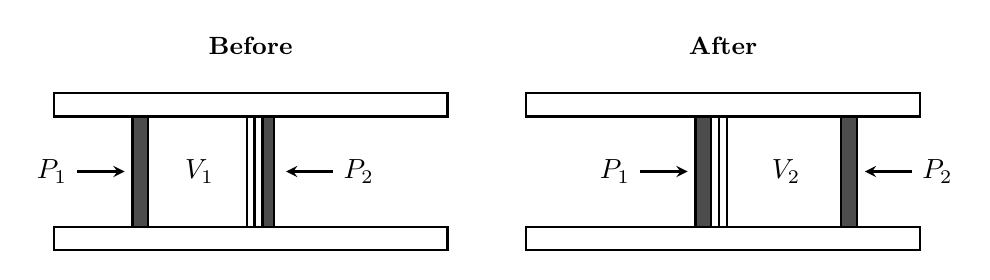
\begin{tikzpicture}[thick]

  %% ---- BEFORE ----
  \node[font=\small\bfseries] at (2.5, 2.6) {Before};

  %% pipe walls
  \draw (0,0) rectangle (5, 0.3);
  \draw (0,1.7) rectangle (5, 2.0);

  %% porous barrier
  \draw (2.45, 0.3) -- (2.45, 1.7);
  \draw (2.55, 0.3) -- (2.55, 1.7);

  %% left piston
  \draw[fill=black!70] (1.0, 0.3) rectangle (1.2, 1.7);

  %% right piston
  \draw[fill=black!70] (2.65, 0.3) rectangle (2.8, 1.7);

  %% labels
  \node at (1.85, 1.0) {$V_1$};
  \draw[->, >=stealth] (0.3,1.0) -- (0.9,1.0);
  \node[left] at (0.3,1.0) {$P_1$};
  \draw[<-, >=stealth] (2.95,1.0) -- (3.55,1.0);
  \node[right] at (3.55,1.0) {$P_2$};

  %% ---- AFTER ----
  \node[font=\small\bfseries] at (8.5, 2.6) {After};

  %% pipe walls
  \draw (6,0) rectangle (11, 0.3);
  \draw (6,1.7) rectangle (11, 2.0);

  %% porous barrier

  \draw (8.45, 0.3) -- (8.45, 1.7);
  \draw (8.55, 0.3) -- (8.55, 1.7);

  %% left piston (pushed all the way to barrier)
  \draw[fill=black!70] (8.15, 0.3) rectangle (8.35, 1.7);

  %% right piston
  \draw[fill=black!70] (10, 0.3) rectangle (10.2, 1.7);

  %% labels
  \node at (9.3, 1.0) {$V_2$};
  \draw[->, >=stealth] (7.45,1.0) -- (8.05,1.0);
  \node[left] at (7.45,1.0) {$P_1$};
  \draw[<-, >=stealth] (10.3,1.0) -- (10.9,1.0);
  \node[right] at (10.9,1.0) {$P_2$};

  

\end{tikzpicture}
\caption{Joule-Thomson process: gas is pushed through a porous barrier from
pressure $P_1$ to $P_2 < P_1$.}
\label{fig:joule-thomson}
\end{figure}

\begin{enumerate}

  \item Show that enthalpy, $H = E + PV$, is conserved.

  \item Find the Joule-Thomson coefficient
    $\mu_{\mathrm{JT}} \equiv \left(\dfrac{\partial T}{\partial P}\right)_{\!H}$
    in terms of $T$, $V$, the heat capacity at constant pressure $C_P$,
    and the volume coefficient of expansion
    $\alpha \equiv \dfrac{1}{V}\!\left(\dfrac{\partial V}{\partial T}\right)_{\!P}$.
    (Hint: You will need to use a Maxwell relation.)

  \item What is $\mu_{\mathrm{JT}}$ for an ideal gas?

  \item If we wish to use the Joule-Thomson process to cool a real (non-ideal)
    gas, what must the sign of $\mu_{\mathrm{JT}}$ be?

  \item Derive $\mu_{\mathrm{JT}}$ for a gas obeying the van der Waals equation
    of state to leading order in the density $N/V$. For what values of
    temperature $T$ can the gas be cooled?

\end{enumerate}

\noindent \underline{\textbf{Solution}} Label all quantities on the left by 1 and quantities on the right by 2. We have 
\begin{equation}
    dH = dH_1+ dH_2 = dE_1 + P_1dV_1 + V_1dP_1 + dE_2 + P_2dV_2 + V_2dP_2. 
\end{equation}
Since the process is adiabatic, we have $dE_i = -\delta W_i = -P_idV_i$. Meanwhile, the pressure is constant; thus, all quantities on the left vanish. Hence, we have $dH=0$. 

Now, consider the temperature $T$ as a function of $H$ and $P$. The total derivative of $T$ is given by
\begin{equation}
    dT = \left(\frac{\partial T}{\partial H}\right)_P dH + \left(\frac{\partial T}{\partial P}\right)_H dP = \left(\frac{\partial T}{\partial P}\right)_H dP \equiv \eta_{\text{JT}}dP.
\end{equation}
Using Maxwell relations, we have
\begin{equation}
    \eta_{\text{JT}} = -\left(\frac{\partial T}{\partial H}\right)_P\left(\frac{\partial H}{\partial P}\right)_T = -\frac{1}{C_P}\left[T\left(\frac{\partial S}{\partial P}\right)_T + V\right] = \frac{1}{C_P}\left[T\left(\frac{\partial V}{\partial T}\right)_P - V\right].
\end{equation}

For ideal gas, 
\begin{equation}
    \left(\frac{\partial V}{\partial T}\right)_P = V \implies \eta_{\text{JT}}=0.
\end{equation}

Since $dP<0$, for a cooling process, $dT<0$, we require $\eta_{\text{JT}}>0$.

The van der Waals equation of state is
\begin{equation}
    \left(P + \frac{aN^2}{V^2}\right)(V-Nb) = NkT.
\end{equation}
Expanding and dropping the $ab$ term as second order in the density $N/V$,
\begin{equation}
    PV - PNb + \frac{aN^2}{V} = NkT.
\end{equation}
Differentiating implicitly at constant $P$,
\begin{equation}
    P\left(\frac{\partial V}{\partial T}\right)_P - \frac{aN^2}{V^2}\left(\frac{\partial V}{\partial T}\right)_P = Nk,
\end{equation}
and so
\begin{equation}
    \left(\frac{\partial V}{\partial T}\right)_P = \frac{Nk}{P - aN^2/V^2} \approx \frac{Nk}{P}\left(1 + \frac{aN^2}{PV^2}\right).
\end{equation}
To leading order in $N/V$ we may replace $V \approx NkT/P$ in the correction term only, giving
\begin{equation}
    \left(\frac{\partial V}{\partial T}\right)_P \approx \frac{Nk}{P} + \frac{aN^2}{kT^2 V}.
\end{equation}
Substituting into the expression for $\eta_{\mathrm{JT}}$ and using $V \approx NkT/P + Nb - aN/kT$ to the same order,
\begin{equation}
    T\left(\frac{\partial V}{\partial T}\right)_P - V 
    = \frac{NkT}{P} + \frac{aN}{kT} - \frac{NkT}{P} - Nb + \frac{aN}{kT}
    = \frac{2aN}{kT} - Nb.
\end{equation}
Hence,
\begin{equation}
    \eta_{\mathrm{JT}} = \frac{N}{C_P}\left(\frac{2a}{kT} - b\right).
    \label{eq:JT-vdW}
\end{equation}
The gas can be cooled ($\eta_{\mathrm{JT}}>0$) only below the \textit{inversion temperature},
\begin{equation}
    T < T_{\mathrm{inv}} \equiv \frac{2a}{kb}.
\end{equation}

\subsection{Adiabatic Compression of Water Near the Triple Point (Imperial 2023 TPSM paper, Q3)}
\label{sec:water-compression}

One gram of pure solid water starts with a temperature and a
pressure both slightly below the triple point of water. The water is compressed
adiabatically to a pressure of 100\,atm. At 1\,atm, the water is found to lie
on the solid--liquid coexistence curve.

You may use the data given at the end of this question.

\begin{enumerate}

  \item Explain what happens as the pressure increases from the starting point
    to 100\,atm and sketch the process on a $PT$ diagram (phase diagram).
    \hfill [8 marks]

  \item Calculate the change in temperature as the pressure increases from
    1\,atm to 100\,atm. \hfill [7 marks]

  \item Writing entropy as a function of $T$ and $P$, show that for a single
    phase,
    %
    \begin{equation}
      d S = \frac{C_P}{T}\,d T - V\beta\,d P,
    \end{equation}
    %
    where $C_P$ is the heat capacity at constant pressure and $\beta$ is the
    thermal expansivity. Hence, for the adiabatic compression, estimate what
    fraction of the water is in the liquid phase at 100\,atm. Comment on any
    assumptions. \hfill [10 marks]
\end{enumerate}

You may assume the following for water:
\begin{itemize}
  \item The specific latent heat of fusion is $334\,\mathrm{J\,g^{-1}}$.
  \item The specific heat capacity at constant pressure of the solid is
    $2.11\,\mathrm{J\,K^{-1}\,g^{-1}}$.
  \item The thermal expansivity of the solid is
    $\beta = 1.65\times10^{-4}\,\mathrm{K^{-1}}$.
  \item The density of the solid is $0.917\,\mathrm{g\,cm^{-3}}$ and the
    liquid is $1.000\,\mathrm{g\,cm^{-3}}$.
  \item The triple point of water is $0.01\,^{\circ}\mathrm{C}$,
    $0.006\,\mathrm{atm}$.
\end{itemize}

\noindent (Note: $1\,\mathrm{atm} = 1.01\times10^{5}\,\mathrm{Pa}$.)
\hfill [Total 25 marks]

\noindent \underline{\textbf{Solution}} The process first starts in the solid region just below the triple point. After an adiabatic thermal compression, it reaches the solid-liquid phase boundary at 1 atm. Then, the pressure further increases following the phase boundary, which means that the solid water turns into liquid water. 

\begin{figure}[htbp]
\centering
\begin{tikzpicture}

  %% ---- Phase boundaries ----
  \draw[black, thick] (0.5,0.2) to[out=60, in=220] (3,2);
  \draw[black, thick] (3,2) to[out=40, in=220] (7,6);
  \draw[black, thick] (3,2) -- (1.96,8.5);

  %% Triple point
  \filldraw[black] (3,2) circle (2pt);
  \node[below right, font=\footnotesize] at (3,2) {triple point};

  %% Region labels
  \node[font=\small\itshape] at (1.5,5)  {solid};
  \node[font=\small\itshape] at (4.2,4)  {liquid};
  \node[font=\small\itshape] at (6.5,3)  {vapour};

  %% ---- Red trajectory ----
  %% Start deep in solid region
  %% Part 1: adiabatic compression — solid red with arrow
  \draw[red, thick, -stealth] (1.8, 1.5) -- (2.68, 4);

  %% Part 2: along coexistence curve — dashed red with arrow
  \draw[red, thick, dashed, -stealth] (2.68, 4) -- (2.2, 7);

  %% Start and end markers
  \draw[red] (1.8,1.5) circle (2.5pt);
  \filldraw[red] (2.2,7) circle (2.5pt);

  %% Labels
  \node[right, red, font=\footnotesize] at (2.3, 2.3)
    {\textcircled{1}};
  \node[left, red, font=\footnotesize] at (2.3, 5.6)
    {\textcircled{2}};

  %% ---- Axes ----
  \draw[-stealth, thick] (0,0) -- (8,0) node[right] {$T$};
  \draw[-stealth, thick] (0,0) -- (0,8) node[above] {$P$};

\end{tikzpicture}
\caption{Schematic $PT$ phase diagram for water (not to scale). The solid
red arrow \textcircled{1} is the adiabatic compression through the solid
region; the dashed red arrow \textcircled{2} tracks the solid--liquid
coexistence curve as ice progressively melts into liquid water.}
\label{fig:PT-schematic}
\end{figure}

Following the Clapeyron equation, we have
\begin{equation}
    \frac{dP}{dT} = \frac{l}{T\Delta v}
\end{equation}
on the solid-liquid boundary. Solving this, we find 
\begin{equation}
    \ln\frac{T_2}{T_1} = \frac{1}{l}\left(\frac{1}{\rho_l}-\frac{1}{\rho_l}\right)\Delta P \implies T_2 = T_1\exp\left[\frac{1}{l}\left(\frac{1}{\rho_l}-\frac{1}{\rho_l}\right)\Delta P\right] = 272.41 \si{K}.
\end{equation}

Now, we write the entropy as $S=S(T,P)$, taking the total derivative, we find
\begin{equation}
    dS = \left(\frac{\partial S}{\partial P}\right)_TdP + \left(\frac{\partial S}{\partial T}\right)_PdT.
\end{equation}
For solid, we can use the Maxwell relation to write the first term as
\begin{equation}
    \left(\frac{\partial S}{\partial P}\right)_T = -\left(\frac{\partial V}{\partial T}\right)_P = -V\beta.
\end{equation}
For the second term, by definition, we have
\begin{equation}
    \left(\frac{\partial S}{\partial T}\right)_P = \frac{C_p}{T}.
\end{equation}
Thus, we find
\begin{equation}
    dS = \frac{C_p}{T}dT - V\beta dP.
    \label{eq:dS}
\end{equation}

Since the whole process is adiabatic, the total change of entropy of the system is zero. Before reaching the phase boundary, the change of entropy is completely governed by (\ref{eq:dS}). After reaching the phase boundary, the total entropy is given by
\begin{equation}
    dS = dS_s + dS_l=0,
\end{equation}
where 
\begin{equation}
    dS_s = \frac{C_p^s}{T}dT - V_s\beta dP \qquad \text{and} \qquad dS_l=\frac{l}{T}dm.
\end{equation}
Since the change of temperature just calculated was very small, we shall take it to be constant on the right-hand sideside. Then, by integration, we find
\begin{equation}
    (1-f)mc_p\ln\frac{T_2}{T_1}- \frac{(1-f)m}{\rho_s}\beta \Delta P = -\frac{fml}{T_2} \implies f= \frac{1}{1+\dfrac{l}{T_1}\left(\dfrac{\beta\Delta P}{\rho_s}-c_p\ln\dfrac{T_2}{T_1}\right)^{-1}} = 0.6\%,
\end{equation}
where $f$ is the fraction of liquid water.

\subsection{Partition Function and Thermodynamics of a Spin-$\frac{1}{2}$ System (David Tong SP, PS1 Q3)}
\label{sec:spin-half}

Consider a system consisting of $N$ spin-$\frac{1}{2}$ particles,
each of which can be in one of two quantum states, `up' and `down'. In a
magnetic field $B$, the energy of a spin in the up/down state is $\pm\mu B/2$
where $\mu$ is the magnetic moment. Show that the partition function is
\begin{equation}
  Z = 2^N \cosh^N\!\left(\frac{\beta\mu B}{2}\right).
\end{equation}

Find the average energy $E$ and entropy $S$. Check that your results for both
quantities make sense at $T=0$ and $T\to\infty$.

Compute the \textit{magnetisation} of the system, defined by $M = N_\uparrow -
N_\downarrow$, where $N_{\uparrow/\downarrow}$ are the number of up/down spins.
The magnetic susceptibility is defined as $\chi \equiv \pd M/\pd B$. Derive
\textit{Curie's Law}, which states that at high temperatures $\chi \sim 1/T$.

\noindent \underline{\textbf{Solution}} First, consider the partition function of a system with a single particle, $z$:
\begin{equation}
    z = e^{-\beta\mu B/2} + e^{+\beta\mu B/2} = 2\cosh\left(\frac{\beta\mu B}{2}\right).
\end{equation}
Assuming the particles are distinguishable (localised on a lattice), the partition function of a $N$ particle system is, therefore,
\begin{equation}
    Z = z^N = 2^N\cosh^N\left(\frac{\beta\mu B}{2}\right).
\end{equation}

The average energy is given by
\begin{equation}
    E  = - \frac{\partial\ln Z}{\partial\beta} = -\frac{\mu BN}{2}\tanh\left(\frac{\beta\mu B}{2}\right),
\end{equation}
and the entropy is
\begin{equation}
    S = k_B(\ln Z + \beta E)
    = Nk_B\left[\ln 2 + \ln\cosh\!\left(\frac{\beta\mu B}{2}\right)
    - \frac{\beta\mu B}{2}\tanh\!\left(\frac{\beta\mu B}{2}\right)\right].
\end{equation}
At $T=0$, $\beta\to\infty$: $\ln\cosh(\beta\mu B/2)\approx \beta\mu B/2$ and $\tanh\to 1$, so the last two terms cancel and $S\to 0$, consistent with a unique ground state.
For $T\to\infty$, $\beta\to 0^+$: $\ln\cosh\to 0$ and $\tanh\to 0$, giving
\begin{equation}
    S \to Nk_B\ln 2,
\end{equation}
the maximum entropy corresponding to all $2^N$ microstates being equally probable.

To compute the magnetisation, let us go back to consider the single particle system. The average magnetisation of such a system is given by
\begin{equation}
    \langle M\rangle = \frac{1}{z}(e^{-\beta\mu B/2}- e^{\beta\mu B/2}) = -\tanh\left(\frac{\beta\mu B}{2}\right).
\end{equation}
The magnetisation of a $N$-particle system is simply
\begin{equation}
    M = -N \tanh\left(\frac{\beta\mu B}{2}\right).
\end{equation}

For large temperature, $\beta\to0^+$, which gives
\begin{equation}
    \chi \approx-\frac{N\beta\mu}{2} \sim \frac{1}{T}.
\end{equation}

\subsection{Heat Capacity of an Interacting Spin System (David Tong Sp, PS1 Q4)}
\label{sec:interacting-spins}

Consider a system of $N$ interacting spins. At low temperatures,
the interactions ensure that all spins are either aligned or anti-aligned with
the $z$ axis, even in the absence of an external field. At high temperatures,
the interactions become less important and spins can point in either
$\pm\hat{z}$ direction. If the heat capacity takes the form
\begin{equation}
  C_V = C_{\max}\!\left(\frac{2T}{T_0}-1\right)
  \quad\text{for } \frac{T_0}{2} < T < T_0
  \quad\text{and}\quad C_V = 0 \text{ otherwise},
\end{equation}
determine $C_{\max}$.

\noindent \underline{\textbf{Solution}} As we have seen in the previous question, the maximum entropy of such a system is given by $Nk_B\ln2$, and the minimum entropy is $0$. By the definition of entropy, we find
\begin{equation}
    \Delta S = Nk_B\ln2 = \int^\infty_0 \frac{C_VdT}{T}.
\end{equation}
Take the heat capacity to be of the form given in the question and evaluate the integral, we find
\begin{equation}
    \Delta S = C_\text{max}(1-\ln2) \implies C_\text{max} = \frac{Nk_B\ln2}{1-\ln2}.
\end{equation}